\section{Results}
\subsection{Hardware}
The results of our hardware setup demonstrated a successful interplay between the Arduino Uno, the Tower Pro MG995R servos, and the serial communication protocol. However, some operational challenges were observed that affected the overall performance.\newline

\subsubsection {Arduino Uno and External Power Supply}

The Arduino Uno, coupled with an external power supply, effectively managed the high-power requirements of the servo motors. It successfully converted control commands from the MATLAB Simulink model into signals for the servos, despite the power limitations of its own microcontroller. This successful integration demonstrated the feasibility of using an Arduino as a central control hub even when the power demands of the system exceed its native capabilities.\newline

\subsubsection{Servo control}

In terms of positional control, the Tower Pro MG995R servos performed commendably within the 3dof Stewart platform setup. They provided a significant level of precision and responsiveness to the Arduino's control signals, consistently rotating and maintaining their output shaft at the required positions.\newline

However, we encountered an issue related to the speed of the servos' response. Despite receiving the correct control signals, the servos showed a delay of about a second before responding, which negatively impacted the real-time control of the platform. This delay was unexpected given the servos' known specifications and introduced additional complexities to the system's performance.\newline

\subsubsection{Serial Communication}

The serial communication protocol facilitated reliable data transmission between the Arduino Uno and the computer running the MATLAB Simulink model. Despite potential latency risks associated with the protocol, the positional data and control commands were consistently transmitted with minimal delay.\newline

However, in relation to the servo response delay, further investigation into the communication block suggested that the issue might lie in the communication between the Arduino and the servos. Despite receiving correct signal frequency at the communication block input, the delay issue persists, indicating that this could be a communication problem between the Arduino and the servos.\newline

\subsection{Ball detection}\label{Ball detection}
The ball detection algorithm has given good results under various brightness conditions, thanks to the auto-brightness adjustment in MATLAB Simulink. We verified the algorithm's effectiveness by testing it with a different webcam, which demonstrated the flexibility of our program.\newline
 During the utilization of the algorithm, no noticeable lag was detected, ensuring a real-time regulation of the ball's position.\newline
\begin{center}
    \begin{figure}[ht!]
        \centering
        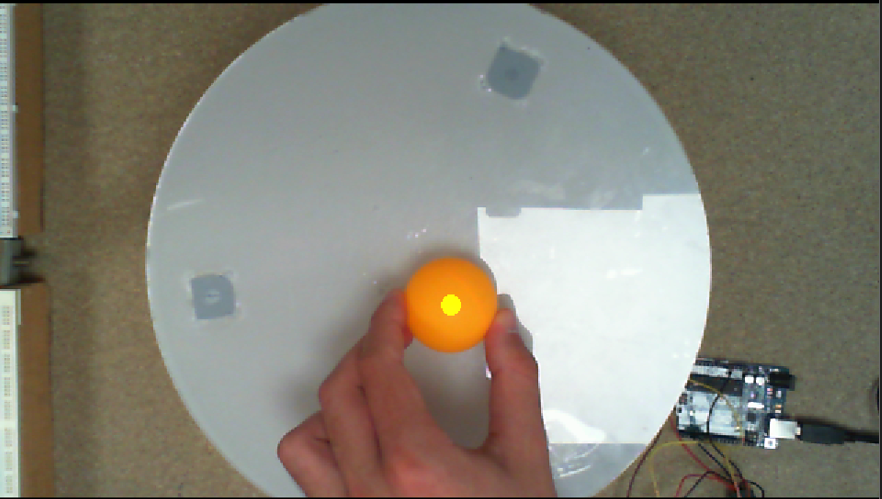
\includegraphics[width=8cm, keepaspectratio]{imports/Pos_BALL_usr.png}
        \caption{Calculated ball position, marked by a yellow circle on the user interface}
    \end{figure}
\end{center}
However, we encountered a minor drawback where the wood support occasionally got misidentified as the ball. Nevertheless, using a x5 zoom on the camera has mitigated much of the issue. Finally, other solutions are evoked in \ref{Ball discussion}. 


\subsection{Simscape model}\label{Simscape model}
After creating a virtual twin of the physical system, a key step was to determine the initial servo angles. It was observed that the angles of the \textit{Revolute Joint} \cite{noauthor_joint_nodate} (servos) were reversed compared to the physical system. Therefore, an important adjustment was made by introducing a negative unit gain to establish the correct angle relationship. Following this adjustment, the digital model exhibited perfect response.

As depicted in Figure \ref{fig:45degreeanimation}, with all setpoint angles set to 45°, the plate appeared perfectly straight.

\begin{center}
    \begin{figure}[ht!]
        \centering
        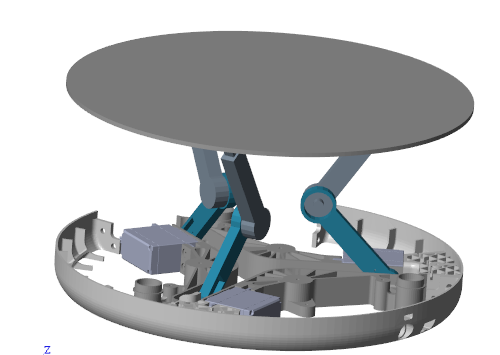
\includegraphics[width=4cm, keepaspectratio]{imports/all_45png.png}
        \caption{3D animation of the digital twin model for setpoint angles all equal to 45°}
        \label{fig:45degreeanimation}
    \end{figure}
\end{center}

As illustrated in Figure \ref{fig:60400angleanimation}, for different setpoint angles (60°, 40°, and 0°), the plate exhibited a tilted position similar to that observed in the real system.

\begin{center}
    \begin{figure}[ht!]
        \centering
        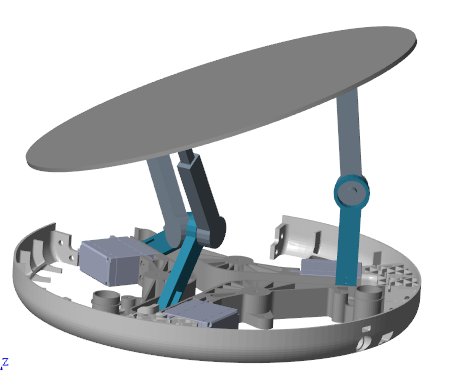
\includegraphics[width=4cm, keepaspectratio]{imports/60_40_0_plate.png}
        \caption{3D animation of the digital twin model for 60°, 40°, and 0° setpoint angles}
        \label{fig:60400angleanimation}
    \end{figure}
\end{center}


\subsection{Controller}

To design the controller, we utilized Simulink to implement the system model described in section \ref{System modeling} By leveraging the sisotool, we obtained insightful results pertaining to the PID constants and the system's behavior. Simulink served as a valuable platform for constructing and simulating the model derived from the theoretical framework outlined in \ref{System modeling}. The model incorporated the relevant system dynamics and allowed us to explore various control strategies. By defining the appropriate transfer functions and input-output relationships, we were able to represent the system's behavior accurately within the Simulink environment.
\\\\
Through the sisotool's graphical interface, we could visualize the system's response to different PID gains and observe the resulting effects on stability, settling time, overshoot, and other relevant performance metrics. By adjusting the PID constants and observing the system's response in real-time, we were able to iteratively fine-tune the controller to achieve the desired behavior.
\\\\
The sisotool allowed us to gain a deep understanding of the interplay between the PID constants and the system's dynamic response. We carefully analyzed the trade-offs between stability and performance, seeking an optimal balance that minimized overshoot, ensured fast response times, and maintained robustness in the face of disturbances or uncertainties.
\\\\
Overall, the combined use of Simulink and the sisotool provided us with a systematic approach to design and optimize the PID controller. The simulation environment enabled us to accurately represent the system's behavior, while the sisotool empowered us to fine-tune the PID constants and achieve a control strategy that met the desired performance criteria.
\\\\
The simulation results yielded insightful findings. However, due to an issue encountered with the physical prototype, its physical implementation was not feasible. Additionally, it is crucial for the controlled system's response to exhibit a restrained nature, avoiding excessive aggressiveness. This consideration is essential as an overly aggressive response could lead to extraordinarily high velocities and accelerations, rendering the system uncontrollable.The system response is as follows:
\begin{center}
    \begin{figure}[ht!]
        \centering
        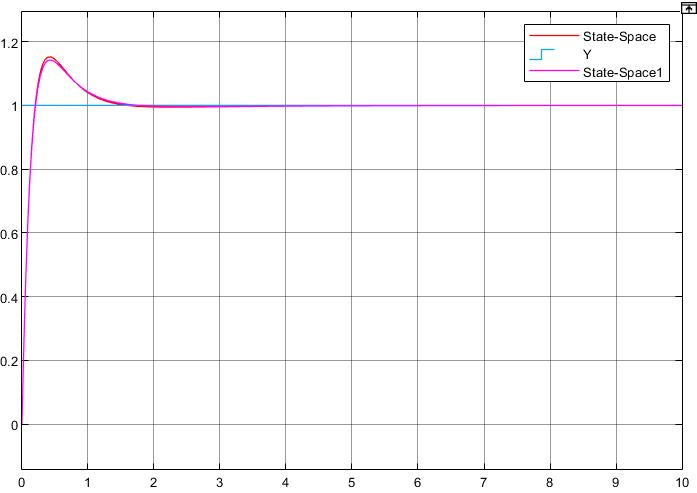
\includegraphics[width=8cm, keepaspectratio]{imports/Captura2.JPG}
        \caption{Modeled system response}
        \label{fig PID result}
    \end{figure}
\end{center}

Considering the requirement for a restrained system response, it is essential to strike a balance between stability and performance. A highly aggressive response may result in rapid and drastic changes in velocity and acceleration, making it difficult to maintain control over the system. By aiming for a more moderate and controlled response, we can ensure that the system remains within manageable limits as we can see in Figure \ref{fig PID result}, allowing for effective control and ensuring the safety and stability of the overall operation.
The optimal gains obtained are as follows: \( k_p = 3.467 \), \( k_i = 1.595 \), \( k_d = 1.414 \).\footnote{The gains \( k_p \), \( k_i \), and \( k_d \) correspond respectively to the parameters \((P)\), \((I)\), and \((D)\) mentioned in Section \ref{Controller Materials} .
}


